%%%% The chapter number should be the numbering of the project  %%%% 
\setcounter{chapter}{0}

%The goal of each bioimage analysis workflow chapter is to let readers to fully understand how image processing and analysis components are used in the workflow and to provide a “design pattern”of workflow. Such understandings will allow readers to modify the workflow for their own purpose, or to use some of those components in other workflow for addressing different types of question. 

\section{Aim}

% This is the trailer of this chapter. A short paragraph summarizing the aim, the motivation, key methods used and the goal. 
The aim of this chapter is to learn how to construct a workflow for measuring the fluorescence intensity localized to the nuclear membrane. For this purpose, the nucleus image is segmented to create a mask along the nuclear rim. The reader will learn a typical technique for automatically delineating the segmented area by post-processing using the mathematical morphology algorithm, and how to loop that piece of ImageJ macro and iterate through multiple image frames to measure changes in fluorescence intensity over time. This chapter is also a good guide for learning how to convert ImageJ macro commands recorded by the Command Recorder to a stand-alone ImageJ macro.  

\section{Introduction}

%Explain the biological background and question why this analysis was designed. If there is any reference that approached the question using image analysis, please cite those papers. Please explain the outline of the workflow.  A block diagram / flow chart of the workflow outline will be quite helpful. 

In some biological research projects, we encounter problems that should be studied by measuring fluorescence intensity at the boundary between two different compartments. Here, we pick up an example analysis that measures the changes in nuclear pore complex (NPC) protein density at nuclear membrane over time, in order to study the translocation process the protein from the cytoplasmic fraction to the nuclear membrane \citep{Boni2015}. 

 We analyze a two-channel time-lapse image stack, a sequence of the process of NPC protein relocalizing from the cytoplasm to the nuclear membrane.  The data was acquired by Andreas Boni (Jan Ellenberg lab, EMBL Heidelberg) and have been used in many training. His work, with more advanced bioimage analysis workflows for analyzing NPC dynamics, is published in The Journal of Cell Biology \citep{Boni2015}. Those codes and image data used in his study, which might be interesting for you after going through this chapter, are accessible through the supplementary data section in the journal website \footnote{http://jcb.rupress.org/content/209/5/705}. 
 
 Two images shown in fig. \ref{fig:NucStrategy} are from the first and the last time points of a time-lapse sequence\footnote{The images shown in the fig. \ref{fig:NucStrategy} are from a 4D hyperstack ``NPC1.tif'', which can be downloaded using ImageJ plugin ``CMCI-EMBL''. More details are in "Dataset" section.}. 

Compare these images carefully. The green signal broadly distributed in the cytoplasm at time point 1 becomes accumulated at the periphery of nuclei (red) at time point 15 - between these image frames, the signal changed it's localization from cytoplasm to the nuclear membrane. We construct a workflow that measures this accumulation process by writing a macro. The workflow involves two steps: First, we segment the rim of nucleus - nuclear membrane - using the first channel (histone). Second, we use that segmented nuclear rim as a mask to measure the intensity changes over time in the second channel. 

\begin{figure}[htbp]
 \centering
 \subfloat[Time point 1]{\label{fig:NucTimePoint1}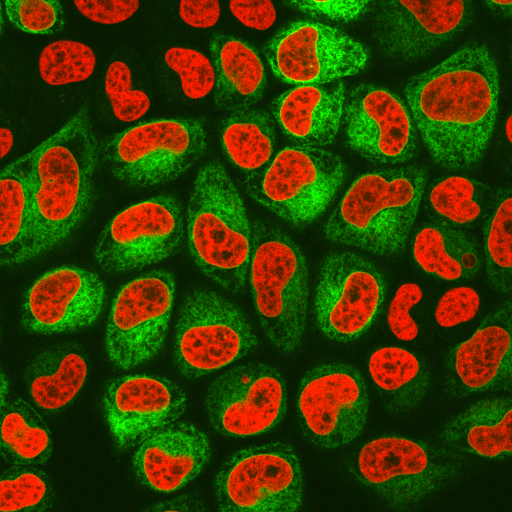
\includegraphics[width = 0.45\textwidth]{fig/NPC_T01.png}} 
 \quad
 \subfloat[Time point 15]{\label{fig:NucTimePoint15}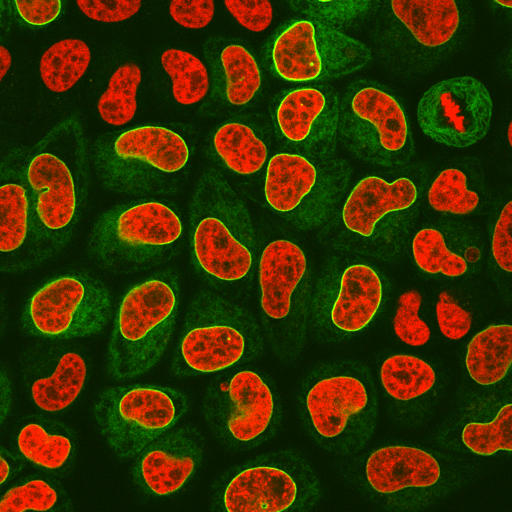
\includegraphics[width = 0.45\textwidth]{fig/NPC_T15.png}} \\
 \caption{NPC localization difference at two time points: More NPC in nucleus periphery. }
 \label{fig:NucStrategy}
\end{figure}

Segmentation of nucleus using its marker (e.g. DAPI) is a popular image analysis technique used in many biological research projects, but to measure more specific location - in our case nuclear membrane - we need to add several more steps to refine the region-of-interest. When we are successful in determining the nuclear membrane, the measurement of intensity in that region over time is rather trivial. We just need to loop the same process for each time point. Especially for the analysis of time-lapse sequence, programming is highly recommended to iterate the measurement for each time point. We use ImageJ macro to put this measurement workflow into an automated script. 

This chapter should be a good guide not only limited to the segmentation of the nuclear membrane, but in general for segmenting the edge (perimeter) of biological compartments such as the edge of organelle, plasma membrane and tissue boundaries. In principle, similar post-processing strategy is also applicable to 3D volumes by using 3D morphology filters. 

\section{Tools}

%List of software packages / plugins / libraries used and brief explanation of how to access / download / install them

We use Fiji (Fiji Is Just ImageJ) for image analysis.

\begin{itemize}
    \item Fiji
    \begin{itemize}
        \item Download URL: \url{https://imagej.net/Fiji/Downloads}
        \item Please choose the latest version. 
        \item No installation of plugin is required. 
    \end{itemize}
\end{itemize}

In addition, a plugin is required for loading the sample image data. Using the``Update sites'' function, please add ``CMCI-EMBL'' to your Fiji installation. Please restart Fiji after this plugin installation. 

\section{Dataset}

%Please upload sample dataset to public servers. ZENODO is the recommended service for this, as the versioning and DOI stamping is available there. 

%Details of the image data. For example, nature of the specimen (e.g. name of the organism), strain if it is known, microscopy and capturing condition details (imaging setup, objective, dt, z-intervals...), type of probe in case of fluorescence image. If someone else has taken the image, please acknowledge and clarify the copyright / licensing. 

All ImageJ macro codes can be downloaded from the Github repository\footnote{https://github.com/miura/NucleusRimIntensityMeasurementsV2/tree/master/code}. 

The image data we used in this chapter can be downloaded using the plugin "CMCI-EMBL". After installation of this plugin, select the menu item \ijmenu{[EMBL > Sample Images > NPCsingleNucleus.tif]} to load the image data. This is a time-lapse sequence of a cell, extracted from ``NPC1.tif'' which can be also downloaded through the same plugin. 

\begin{itemize}
\item Cell Type: 
\item Scale: 
\item Frame Rate: Sec / Frame
\item Channels
\begin{itemize}
    \item Red channel: Histon, ex/em 358/461nm \dots
	\item Green Channel: NPC,  ex/em 358/461nm \dots
\end{itemize}
\end{itemize}

\section{Workflow}

%Please upload the full code to Github and link the repository in this chapter. 

%Step-by-Step explanation of the workflow should be provided along with the corresponding part of the code.  The algorithm of each component is expected to be explained how it is working. If the algorithm is a famous one, it will be OK by providing a reference such as Gonzalez & Woods textbook and the page number. 

% please add one or two exercises per subsection (subsection = a block within workflow), to check the understanding of the reader.  

%\section{Measurement of Nucleus Periphery Intensity}

To simplify the development, we focus on a single cell / nucleus to construct the workflow. Load the image stack \textbf{NPCsingleNucleus.tif}. This is a hyperstack sequence. Slide the scroll bar at the bottom back-and-forth to watch the process of intensity changes. Histone signal (red), used as a marker for nucleus, is more or less constant with its distribution. On the other hand, the NPC signal (green) exhibits strong accumulation to the nuclear membrane. To study this accumulation process, our aim is to measure the intensity changes of green signal intensity at the rim of the nucleus over time. The outline of the workflow is shown in the diagram (Fig.\ref{fig:outline}). 

\begin{figure}[H]
\begin{center}
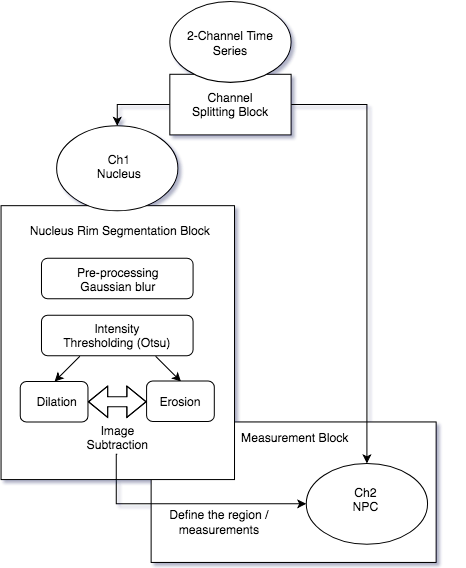
\includegraphics[scale=0.9]{fig/nucrimMeasurementsDiagram.png}
\caption{Outline of the workflow.}
\label{fig:outline}
\end{center}
\end{figure}

To achieve this aim we first need to identify the region of nucleus rim (``segmentation'') - in other words, we create a mask of the nucleus rim. Using this mask we measure the changes in intensity over time. 

\subsection{Segmentation of Nucleus Rim}

We first write a macro for the nucleus rim segmentation by taking following steps:  

\begin{enumerate}
  \item Split the original multi-channel image stack and create two image stacks of each channel for processing them independently (fig. \ref{fig:originalNucleus})
  \item Blur the image to attenuate noise (fig. \ref{fig:BlurredNucleus})
    \item Nucleus segmentation: Binarize the image by intensity thresholding  (fig. \ref{fig:BInarizedNucleus})
    \item Remove other Nuclei: At the right-bottom corner of the image, a small part of different nucleus is present. This should be removed. 
    \item Duplicate the image
    \begin{enumerate}
        \item Erode the original (fig. \ref{fig:erodedBinary})

        \item Dilate the duplicated (fig. \ref{fig:dilatedBinary})

    \end{enumerate}
    \item Subtract the eroded from the dilated (fig. \ref{fig:NucleusRim})

\end{enumerate}

\begin{figure}[!ht]
 \centering
 \subfloat[Original Nucleus Image]{\label{fig:originalNucleus}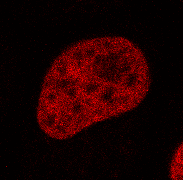
\includegraphics[width = 0.30\textwidth]{fig/OriginalNuc.png}} 
 \quad
 \subfloat[Blurred Nulcleus Image]{\label{fig:BlurredNucleus}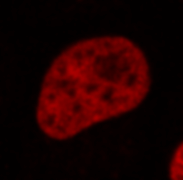
\includegraphics[width = 0.30\textwidth]{fig/BlurredNuc.png}}
 \quad
 \subfloat[Binarized image, after thresholding.]{\label{fig:BInarizedNucleus}
\includegraphics[width = 0.30\textwidth]{fig/ConvertedMask.png}} \\
 \subfloat[Dilated Binary Image]{\label{fig:dilatedBinary}
\includegraphics[width = 0.30\textwidth]{fig/dilated.png}}
 \quad
 \subfloat[Eroded Binary Image]{\label{fig:erodedBinary}
\includegraphics[width = 0.30\textwidth]{fig/eroded.png}}
 \quad
 \subfloat[Subtraction Result, the rim.]{\label{fig:NucleusRim}
\includegraphics[width = 0.30\textwidth]{fig/NucRim.png}}
 \caption{Strategy of measurement.}
 \label{fig:nucsegProc}
\end{figure}


In the following we record these steps as macro commands using the Command Recorder (\ijmenu{[Plugins > Macros > Record\ldots]}). We recommend you NOT to launch the command recorder from the beginning. Please first try to reproduce the workflow using mouse and the graphical user interface (GUI). This is like a rehearsal before recording your actions. When you become clear with the steps you have to take, record the processing steps. When you use the command recorder, be sure that ``Macro'' is selected in the ``Record:'' drop down menu at the top-left corner of the recorder.

\subsubsection{Block 1: Splitting Channels}

To split the multichannel image stack from the GUI menu, do \ilcom{[Image > Color > Split Channels]}. In the Recorder you will see the following command. 
\begin{lstlisting}[numbers=none]
run("Split Channels");
\end{lstlisting}

\ilcom{run} function is the most frequently used build-in macro function. 

\fbox{
\parbox[b][15em][c]{0.80\textwidth}{
  \textbf{run("command"[, "options"])}
  Executes an ImageJ menu command. The optional second argument contains values that are automatically entered into dialog boxes (must be GenericDialog or OpenDialog). Use the Command Recorder (Plugins>Macros>Record) to generate run() function calls. Use string concatenation to pass a variable as an argument. With ImageJ 1.43 and later, variables can be passed without using string concatenation by adding "\&" to the variable name.
}}

The run function takes a menu item as the first argument and optional values (values you fill-in in a dialog window) in the second argument. In case of channel splitting, there is no such optional value so the second argument is ignored. 

We then process the nucleus image. Click the nucleus image window to bring it up to the top - We call this action as ``activating a window''. By this clicking, we activated Channel 2 (red, nucleus image).

Please confirm that a new command shown below, is added to the recorder after activating the nucleus image.

\ilcom{selectWindow("C1-NPCsingleNucleus.tif");}

\dots  Here is the explanation from the macro function reference. 

\fbox{
\parbox[b][3em][c]{0.80\textwidth}{
  \textbf{selectWindow("name")}\\
Activates the window with the title "name".
}
}

This function takes a window title as an argument and activates a window with that title. When we used mouse to activate the nucleus channel window, we did it manually by visually recognizing the red nucleus image. On the other hand, in macro, we need to know the title of the windows of each individual channels to activate a specific window to provide it to macro as an argument of ``selectWindow''command. How can we get the name of the nucleus channel window after splitting the channels of the original image?

Standard behavior of ``Split Channel'' command is that it automatically names the resulting stacks of individual channels by prefixing ``C1-'' or ``C2-'' or ``C3'' to the original image title. Based on this known behavior, we can construct these names if the original image title is known. For this we use the command \ilcom{getTitle()} which returns the title of currently active window as a string. 

\fbox{
\parbox[b][3em][c]{0.80\textwidth}{
\textbf{getTitle()}\\
Returns the title of the current image.
}
}

Here is the code to activate the nucleus channel automatically after the splitting. More importantly, we also acquire ``image ID''. This will be explained later.  


\lstinputlisting[morekeywords={*, getImageID, selectWindow, run, getTitle}]{code/code_block1_ChannelSplitting.ijm}


\textbf{Details:} 
\begin{itemize}
\item The first line grabs the window title as a string variable ``orgName''. 
\item The second line splits the stacks to each individual channel stack.
\item 3rd and 4th lines compose the window title for each channel stack. 
\item 5th line activates the channel 1 stack. 
\item 6th line acquires the image ID of channel 1 stack. 
\item 7th line activates the channel 2 stack. 
\item 8th line acquires the image ID of channel 2 stack. 
\end{itemize}


In lines 6 and 7, we acquire \textbf{image IDs}. Here is some more explanation about this: Each window has a unique ID number. To get this ID number from each image we use the command \ilcom{getImageID()}.

\begin{indentCom}
\fbox{
\parbox[b][8em][c]{0.80\textwidth}{
\textbf{getImageID()}\\
Returns the unique ID (a negative number) of the active image. Use the selectImage(id), isOpen(id) and isActive(id) functions to activate an image or to determine if it is open or active.
}
}
\end{indentCom}

A window can be activated by \ilcom{selectWindow} using its window title, but this could have a problem if there is another window with same name. Image ID has less problem since it is uniquely given to each window. To select a window using image ID, we use \ilcom{selectImage(ID)} command.

\begin{indentCom}
\fbox{
\parbox[b][8em][c]{0.80\textwidth}{
\textbf{selectImage(id)}\\
Activates the image with the specified ID (a negative number). If id is greater than zero, activates the ID-th image listed in the Window menu. The ID can also be an image title (a string).
}
}
\end{indentCom}

We acquire image IDs just after the splitting. From here on, we will use image IDs when we want to specify the image window we want to work on and to activate it. 

\begin{indentexercise}{1}
Test the code below and run it on several image windows. Confirm that each window has an unique ID number. 
%\begin{lstlisting}[numbers=none]
\begin{lstlisting}
id = getImageID();
print( id );
name = getTitle();
print( name );
\end{lstlisting}
\end{indentexercise}

Save the channel splitting macro. When you name the file, add an extension ``.ijm'', as this indicates that the file is an ImageJ macro. This is only a part of the final workflow, and we call such part as a \textbf{``block''} of the workflow, and by assembling blocks with various functions, we construct a \textbf{workflow}. A block is a functional unit within the workflow. Each block is consisting of several \textbf{components}, each of which is the build-in function that implements a certain algorithm.  

In the current case, we just finished the \textbf{Channel Splitting Block}, consisting of a channel splitter component, a window title getter component, an image window ID getter component, and window selector components. 

\subsubsection{Block 2: Segmentation of Nucleus Rim}

Now we start working on the segmentation of nucleus rim. For this, we use only the nucleus image stack (channel 1) we got in the Block 1. Create a new tab in the script editor by \ilcom{[File > New]}. We use this blank editor to  write the next \textbf{block} for the detection of nucleus rim. We assemble all blocks as a single workflow later. 

Following is the step-by-step procedure. Try first using the GUI (your mouse and the menu bar!). Then launch the Command recorder, redo the steps to record the history of commands. I recommend you to do so mainly because the initial trials with GUI let you visually understand what is going on, and also to get used to the sequence of operation for the command recording. 

\begin{enumerate}
  \item Gaussian Blur
  \begin{itemize}
    \item \ijmenu{[Process > Filter > Gaussian Blur]}, sigma = 1.5, tick ``Do Stack''
    \item This diminutive blurring of the image attenuates noise and allows a better result for the segmentation.  
  \end{itemize}
  \item Find Threshold
  \begin{itemize}
    \item \ijmenu{[Image > Adjust > Threshold]},  select Otsu method
    \item This simply changes the LUT, but not the data 
  \end{itemize}
  \item Apply Threshold: Click 'Apply'
  \begin{itemize}
    \item Changes the data to black and white using the threshold value using the Otsu method. 
  \end{itemize}
  \item Find Threshold again (Otsu method)
  \begin{itemize}
    \item We do this again for selecting the nucleus for the ``AnalyzeParticle'' in the following step.
  \end{itemize}
  \item Analyze Particles
  \begin{itemize}
    \item \ijmenu{[Analyze > Analyze Particles]}
    \item Options:
    \begin{itemize}
      \item Size: 800-Infinity
      \item Tick ``Pixel Units''
      \item Circularity: default (0 - 1.0)
      \item Show: Mask
      \item Tick Display Results, Clear results, Exclude on edges, Include holes. 
    \end{itemize}
    \item We use AnalyzeParticle as a filter for segmented object. In our case, this filtering removes nucleus touching the edge of image. This way of usage is also effective in removing small none-nucleus signals. 
  \end{itemize}
  \item Invert the LUT of the "Mask" created by AnalyzeParticle, so operations done below recognizes nucleus as the target of Dilation and Erosion. 
  \begin{itemize}
    \item \ijmenu{[Image > Look-up Table > Invert LUT]}
  \end{itemize}
  \item Duplicate the "Mask" Stack, and then apply "Dilation" to one stack and apply "Erosion" to the duplicated.
  \begin{itemize}
    \item \ijmenu{[Image > Duplicate]}
    \item Set Iterations \ijmenu{ [Process > Binary > Options]}
    \begin{itemize}
      \item iterations 2 or 3
      \item dark background
    \end{itemize}
    \item Original: Dilate \ijmenu{[Process > Binary > Dilate]}
    \begin{itemize}
      \item This increases the edge of nucleus by 2 or 3 pixels. 
    \end{itemize}
    \item Duplicate: Erode \ijmenu{[Process > Binary > Erode]}
    \begin{itemize}
      \item This decreases the edge of nucleus by 2 or 3 pixels. 
    \end{itemize}
  \end{itemize}
  \item Image Subtraction
  \begin{itemize}
    \item \ijmenu{[Process > Image Calculator]}
    \item tick ``keep original'', compute the difference of Dilated and Eroded.
    \begin{itemize}
      \item Leaves a band of 4 or 6 pixels at the edge of nucleus. 
    \end{itemize} 
  \end{itemize}
\end{enumerate}

When you are done with the macro recording, check the results in the recorder. Below is an example of the output from the recorder. 

\lstinputlisting{code/code_block2_recordNucSeg.ijm}

This recorded macro already runs properly as it is, but there is a problem: the code works only with image data with a specific window title. See the line 1. The command looks like this.   

\ilcom{selectWindow("C1-NPCsingleNucleus.tif");}. 

The window title given in the argument of \ilcom{selectWindow} is hard-coded, so that if you need to apply this macro to a image data with a different window title, it will not work. The macro
needs to be improved to allow the general applicability to other images. 

For this reason, we need to change the code so that it uses ImageID instead of a fixed image title. Since the ImageID of the nucleus channel was already acquired after splitting the original image, we can use that ID to activate a specific image window. 

As we are working separately from the channel splitting block, we assume that the nucleus channel stack is active and is the top window at the starting of current code. We replace the first line \ilcom{selectWindow} with \ilcom{getImageID()} command to capture the ID number of the nucleus image window. Next, we need to add \ilcom{getImageID} in line 10 and 13 to capture IDs of newly created windows. Due to these changes, we need to replace \ilcom{selectWindow} in line 12 and 15 to \ilcom{selectImage} to consistently use ImageID for accessing specific window. After these replacement, the updated code will look like the one shown below. 


\lstinputlisting[morekeywords={*, getImageID, selectImage, orgID, dilateID, erodeID}]{code/code_block2_recordNucSegV2.ijm}

Here is the explanation of what was done. 
\begin{itemize}
  \item line 1: The first line is replaced with the \ilcom{getImageID()} command. 
  \item line 10: \ilcom{getImageID()} command was inserted for a new image created by Analyze Particle command (in line 9). The new image is the mask that is eliminated with edge-touching nucleus. 
  \item line 13: \ilcom{getImageID()} command was inserted for the duplicated image. 
  \item line 15: The \ilcom{selectWindow} command in line 14 was commented out and replaced by the \ilcom{selectImage} command. 
  \item line 19: \ilcom{selectWindow} command is replaced by the \ilcom{selectImage} command. 
  \item line 22: Because we now have ImageIDs of both dilated and eroded images, we replace the titles of image windows with imageIDs for image calculator arguments. Compare the line 21 (commented out) and the line 22. 
\end{itemize}

We are now almost done with the generalization of the nucleus rim segmentation block, but there still is a part that can be more general instead of a fixed window name. See line 12. This line uses \ilcom{run} command to duplicate the "Mask" stack. 

\ilcom{run("Duplicate...", "title=[Mask of C1-NPCsingleNucleus-1.tif] duplicate range=1-15");}

The first argument ``Duplicate\ldots'' is the name of the menu item \ijmenu{[Image > Duplicate\ldots]} and this is OK. 

The second argument contains multiple optional values you chose in the GUI. The first is the title of the duplicated image, that was automatically created by suffixing ``-1'' to the image title. Square brackets surrounding this new image title is for avoiding the problem with spaces in the image title, because spaces are used as the separator for the options in the second argument. ``duplicate'' is a keyword of a checkbox in the duplication dialog, for choosing whether to duplicate multiple frames in a stack or just a single currently shown frame. The third option is the frame range (\ilcom{range=}), which defines the range of frames to be duplicated. Since we want to duplicate all frames, the range is set to \ilcom{1-15}, from the first frame to the last 15th frame.

Within this second argument, two values in this command are not flexible enough for applying the macro to other images with different names. First is the image title. We better have a more general name for the duplicated image. The second is the frame range. The duplication of full stack is better be applicable for stacks with any number of frames, not limited to 15-frames stacks. 
We can construct the option string of the second argument as shown below to allow the general applicability of the macro. 

\ilcom{options = "title = dup.tif duplicate range=1-" + nSlices}

\ilcom{nSlices} is a macro function that returns the number of frames or slices in the current stack. It allows to duplicate all frames of a stack, regardless of the number of frames within that stack. 

We can now replace the second argument for image duplication by this new variable "options". 

\ilcom{run("Duplicate...", options);}

\begin{indentexercise}{2}
Create a new script tab and write the code below. Run the code with various stacks with different slice or frame numbers and confirm that this short macro successfully duplicate stacks with any slice or frame numbers. 
\begin{lstlisting}
print(nSlices);
options = "title=dup.tif duplicate range=1-" + nSlices;
print(options);
run("Duplicate...", options);
\end{lstlisting}
\end{indentexercise}

Below is the upgraded code. All the lines previously commented out were removed, and line 10 was inserted for preparing options for the \ilcom{run("Duplicate} command. In addition, we added line 19 - 24 for closing all images that were used for getting the image math results. 

\lstinputlisting{code/code_block2_recordNucSegV3.ijm}

We now have a block that segments nucleus rim. Save this code, and we are done with the second block of the workflow. 

\subsection{Block 3: Intensity Measurement using Mask}

Using the isolated nucleus rim image, we can specify the region for measuring the fluorescence intensity in the NPC channel. This will be the third block of the workflow. 

Before start writing the third block of the workflow, we do a small preparation. We merge the rim-segmented stack and the NPC stack to create a multi-channel stack, which will be used as the input image data of this third block. Open the rim binary image (if you closed it already, run the second block macro again to regenerate it!) and the NPC image.  

\begin{figure}[!ht]
\begin{center}
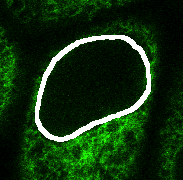
\includegraphics[scale=1.0]{fig/NucRimNPTMerged.png}
\caption{Segmented rim and NPC channel merged.}
\label{fig:NucRimMerged}
\end{center}
\end{figure}

Two stacks can be merged to a two channel image stack by the following command.  

\ilcom{[Image > Color > Merge Channels\ldots]}

In the dialogue window, assign red color (C1) to the nucleus channel (nucleus rim binary image), and  green color (C2) to the NPT channel. Make sure that "Create composite" is ticked. Clicking ``OK'' button, you will have an image stack that looks like figure \ref{fig:NucRimMerged}.

\begin{figure}[!ht]
\begin{center}
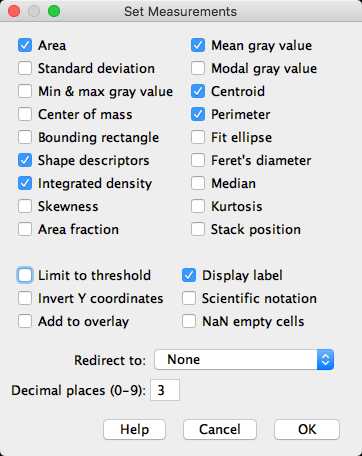
\includegraphics[scale=0.5]{fig/SetMeasurements.png}
\caption{Measurement Settings.}
\label{fig:MeasSetting}
\end{center}
\end{figure}

We are now ready to start writing the third block of the workflow. Please follow the steps below using GUI. When you become sure with the operations, record your operations using Command Recorder.   

\begin{enumerate}
  \item \ijmenu{[Image > Color > Split Channels\ldots]}
  \item \ijmenu{[Analysis > Set Measurements\ldots]}
  \begin{itemize}
    \item You will see a dialog window with many check boxes (Fig. \ref{fig:MeasSetting}). Among the parameters to be measured, tick at least \ilcom{Area, Mean gray value} and \ilcom{Integrated density}. Integrated density is the sum of all pixel values. 
  \end{itemize}
  \item Activate the rim image and do \ijmenu{[Edit > Selection > Create Selection]}
  \begin{itemize}
    \item This selects the background, not the rim. 
  \end{itemize}
  \item \ijmenu{[Edit > Selection > make Inverse]}
  \begin{itemize}
    \item Inverting the selection, now we are selecting the nucleus rim. 
  \end{itemize}
  \item Activate the NPC image (C2) and then [Edit > Selection > Restore Selection]
  \begin{itemize}
      \item 
  \end{itemize}
  \item \ijmenu{[Analyze > Measure]}
\end{enumerate}

Selection of the rim should look like figure \ref{fig_RoiNucRim}.

\begin{figure}[ht!]
\begin{center}
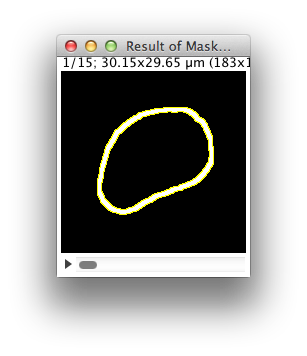
\includegraphics[scale=0.8]{fig/ROIselectionNucRim.png}
\caption{ROI selection of nucleus rim. }
\label{fig_RoiNucRim}
\end{center}
\end{figure}

You will then see results in the Results table such as shown in figure \ref{fig_NucRimMeasureResults}.

\begin{figure}[h!]
\begin{center}
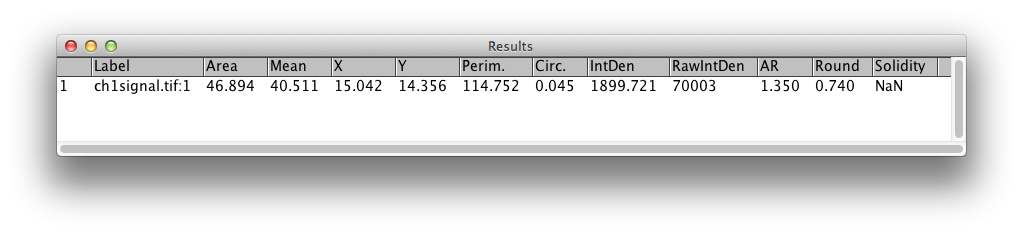
\includegraphics[width=0.95\textwidth]{fig/MeasurementResults.png}
\caption{Results output.}
\label{fig_NucRimMeasureResults}
\end{center}
\end{figure}

When you record these procedures by Command Recorder, the code will look like shown below. Create a new tab in the Script Editor and copy \& paste (or it's possible to do the same by clicking ``create'' button in the Recorder).

\begin{lstlisting}
run("Split Channels");
run("Set Measurements...", "area mean centroid perimeter shape integrated display redirect=None decimal=3");
selectWindow("C1-Composite");
run("Create Selection");
run("Make Inverse");
selectWindow("C2-Composite");
run("Restore Selection");
run("Measure");
\end{lstlisting}

In the 1st line, we split the multichannel stack to do processing individually. In the 3rd and the 6th lines, specific window titles are used. Just like we did in the first block, we need to convert these lines by composing window title of stacks for individual channel by adding prefixes. We also need to acquire their image IDs. For composing window titles, we just need to reuse the code we wrote already in the section ``Block 1: Splitting Channels''. 


\lstinputlisting[morekeywords={*, c1name, c2name, c1id, c2id, opt, getTitle}]{code/code_block3_measurements.ijm}


\begin{itemize}
    \item Line 1: We first need to capture the title of the multi-channel image. 
    \item Line 2: Then the channels are separated into two stacks.
    \item Line 3-4: Since we know the rule of how the resulting image stack names are, we construct titles each for channel 1 and channel 2. 
    \item Line 5-8: We then acquire image IDs.
    \item Line 9-10: To be more explicit, we compose the measurement options as \ilcom{opt} in line 9 and then use that variable \ilcom{opt} as an argument for \ilcom{Set Measurements} in line 10.
    \item Line 11: Activate nucleus rim image using ImageID captured in line 6, instead of using \ilcom{selectWindow}.
    \item Line 12-13: Create nucleus rim ROI (a selection).
    \item Line 14: Activate NPC image using ImageID captured in line 8.
    \item Line 15: Restore the ROI created in line 13.
    \item Line 16: We measure the region specified by the ROI created above.
\end{itemize}

\begin{indentexercise}{3}
Merge the nucleus rim and the NPC image stacks as described in the beginning of this section and test the code

\ilcom{code\_block3\_measurements.ijm} 

to measure the fluorescence intensity of the nuclear rim. 
\end{indentexercise}

\subsection{Integration: The measurement over time}

The code above measures only one frame. To measure the intensity changes over time, we need to add \textbf{looping} from line 11 to 16 in \ilcom{code\_block3\_measurements.ijm} to repeat the measurement over time frames. For this, we need to modify the code by adding a \textbf{for-loop}.

\lstinputlisting[morekeywords={*, for, nSlices, setSlice}]{code/code_block3_MeasurementOverTime.ijm}

In this updated code, following 4 lines were added for looping through the time lapse frames and measure successively. 
\begin{itemize}
    \item A new line was inserted at line 11 to define the condition of for-looping.
    \item A new line was inserted at line 13 to activate a specific frame in the nucleus rim stack.
    \item A new line was inserted at line 17 to activate a specific frame in the NPC stack.
    \item A curly brace was added at line 20 to close the looping.
\end{itemize}

\begin{indentexercise}{4}
Merge rim and NPC image stacks and test the code 

\ilcom{code\_block3\_MeasurementOverTime.ijm} 

to see if it measures the intensity of nucleus rim over time frames. 

If you see 15 lines of measurement values in the Results window, you are successful. 
\end{indentexercise}

\subsection{Integrating Segmentation and Measurements}

Finally, we can assemble three blocks of code: the channel splitting block, the segmentation block and the intensity measurement block. As the third block, the intensity measurement block, starts with a two-channel stack (nucleus rim segmentation image and the NPC signal image), all we need to do is to insert the segmentation block between line 4 and line 5 of block 3 code \ilcom{code\_block3\_MeasurementOverTime.ijm}. 

Instead of copy and pasting the segmentation block to the measurement block, a better way to do this is to convert the segmentation block to a user-defined function. Like all the macro commands that you see in the Build-in ImageJ macro function reference, we can create our own function by ourselves. We briefly learn how to write a custom function with a simple example. 

If we have a code like below:

\begin{lstlisting}
a = 10;
b = 20;
c = a + b + a * b ;
print( c );
\end{lstlisting}

Evidently, "230" will be printed in the log window. Now, We can convert this formula to a custom function \ilcom{calc1} that does the calculation in line 3.

\begin{lstlisting}[morekeywords={*, function, return}]
a = 10;
b = 20;
c = calc1(a, b);
print( c );

function calc1(n, m){
	return n + m + n * m;
}
\end{lstlisting}

Three lines were added to the original code. Line 6 declares a new user-defined function named ``calc1''. It takes two arguments, \ilcom{n} and \ilcom{m}.  Commands between curly braces is the content of this function, and in this case there is only one line that returns a value. To be more explanatory, this function can be rewritten as follows to do the same thing. 

\begin{lstlisting}[morekeywords={*, function, return}]
function calc1(n, m){
    answer = n + m + n * m;
	return answer;
}
\end{lstlisting}

\begin{indentexercise}{5}
\begin{enumerate}
\item Modify the code above so that the function \ilcom{calc1} calculates m to the power of n. Use the build-in command pow(m, n). 

\item Change the name of function to \ilcom{calc2} and run the code. If there is error, fix the code. 
\end{enumerate}

\end{indentexercise}

In a similar way, we can convert the segmentation block to a single custom function that takes an ImageID as input, does pre-processing, does segmentation, and then returns an ImageID of the segmented image as the output. Here is the code: 

\lstinputlisting[morekeywords={*, function, return, orgID, resultID, nucseg}]{code/code_block2_recordNucSegV3_function.ijm}

Only several lines were added to the original \ilcom{code\_block2\_recordNucSegV3.ijm}. 

\begin{itemize}
    \item In line 1, we declare that this is a custom function named \ilcom{nucseg} that takes a single argument \ilcom{orgID}. In the original code, orgID, which is the imageID of the histone channel image, was captured using \ilcom{getImageID} command. 
    \item Line 2 is commented out. This is because We do not need to do \ilcom{getImageID} since the imageID of the  histone channel image is provided through the argument of the function.  
    \item One line is inserted at line 20, to capture the imageID of the resulting image stack - the mask of nuclear rim - of Image Calculation in line 19. This imageID is named as a variable ``resultID'' in the function and is returned in the line 28 as the final output of the function.
    \item \ilcom{run("Clear Results");} is added at the bottom (line 27) to clear the results table, as we want to have only the results of intensity measurement later.
    \item  In the last line, a curly brace is added to mark the boundary of function.
\end{itemize}

We can paste this function \ilcom{nucseg( orgID )} below the intensity measurement macro, and call this function to segment the nucleus rim. In below, I show only the part in the block 3 intensity measurement where function call was added. line 7 to line 8 was inserted to \ilcom{code\_block3\_MeasurementOverTime.ijm}. 

\begin{lstlisting}
orgName = getTitle();
run("Split Channels");
c1name = "C1-" + orgName;
c2name = "C2-" + orgName;

selectWindow(c1name);
nucorgID = getImageID();
nucrimID = nucseg( nucorgID );

selectWindow(c2name);
c2id = getImageID();
opt = "area mean centroid perimeter shape integrated display redirect=None decimal=3";
run("Set Measurements...", opt);
for (i =0; i < nSlices; i++){
    selectImage( nucrimID );
    setSlice( i + 1 );
    run("Create Selection");
    run("Make Inverse");
    selectImage( c2id );
    setSlice( i + 1 );
    run("Restore Selection");
    run("Measure");
}
\end{lstlisting}

In line 6 and 7, the image ID of the nucleus (histone) channel is captured. As we do not know if the nucleus channel image stack is the top window, we explicitly call it to the top by \ilcom{selectWindow}, and then get its ImageID. This ImageID \ilcom{nucorgID} is then passed to the segmentation function in line 8 (\ilcom{nucseg(nucorgID)}). 

After the image segmentation is done in the function \ilcom{nucseg}, the ImageID of segmentation result is returned. We capture this ImageID by a variable \ilcom{nucrimID}. From there, everything is same like we already coded, except that the image selection at line 15 now uses \ilcom{nucrimID}.  

Here is the final code. 

 \lstinputlisting[morekeywords={*, function, return, orgID, resultID, nucseg}]{code/code_final.ijm}


\section{Results and Conclusion}

% Please present the final results, and provide an example of how one can present and interpret that results. Please also add a conclusion of the chapter. 
\begin{figure}[h!]
\begin{center}
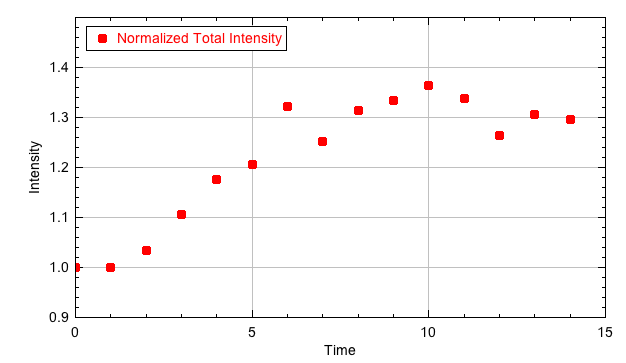
\includegraphics[scale=0.4]{fig/totalIntensityPlot.png}
\caption{Changes in the Total Fluorescence intensity over time}
\label{fig:FluorescenceChangeOvertime}
\end{center}
\end{figure}

The final output is a list of nucleus rim intensity values for each time point in Results window. These values can be saved in a CSV file and further analyzed using other software tools more suited for data analysis such as R or Python. Here, to summarize the analysis in this chapter, we plot the changes in the total fluorescence intensity over time using ImageJ Macro \ilcom{code\_plotResults.ijm} (Fig. \ref{fig:FluorescenceChangeOvertime}). The code appears after the paragraph below. 

The plot in Fig.\ref{fig:FluorescenceChangeOvertime} shows an increase in total fluorescence intensity by 1.3-folds in the initial five time points, and then it becomes mostly constant . To know the baseline level intensity more precisely, it might be better to start the imaging and measurement from an earlier time point. In addition, ideally, more measurements could be done with other nuclei to compute an averaged curve for a more reliable results. 

Here is the code for this plotting. Explanations follow. 

 \lstinputlisting[morekeywords={*, newArray, nResults, getResults. Array, getStatistics, getSequence, Plot, create, setLimits, setColor, setLineWidth, add, setFontSize, addLegend }]{code/code_plotResults.ijm}
 
 \begin{itemize}
     \item Line 2 creates a new array for storing intensity measurements listed in the Results table. \ilcom{nResults} is a build-in function that returns number of rows in the table. This array will be the Y-axis value in the plot. 
     \item Line 3-4 gets the result of non-calibrated integrated density (Column "RawIntDen") of each row, and divide that value by the integrated density at the time point 0 (the first frame). 
     \item Line 7 creates a new array for X-axis values, where we will store time points. To simplify, we use the frame number as time points, starting from 0. 
     \item Line 10: For fitting the plot in a good range, we first get the minimum and the maximum values of measured intensity. With function \ilcom{Array.getStatistics}, descriptive statistics values are called back to the provided variables in the argument. In this case, \ilcom{amin} is the minimum value and \ilcom{amax} is the maximum value of the array. 
     \item Line 13-19: Plotting commands.
     \begin{itemize}
         \item Line 13 creates the plot with specified title, X-axis label and Y-axis label. 
         \item Line 14 sets the range of values to be shown in the plot. Here, the minimum and the maximum value of measurement results are used.
         \item Line 15 sets the color of the marker.
         \item Line 16 sets the line width of the marker.
         \item Line 17 sets the shape of the marker, X-axis values (the array \ilcom{t}) and Y-axis values (the array \ilcom{intA})
         \item Line 18 sets the font size of the title and labels
         \item Line 19 adds the legend of the plot.  
     \end{itemize}
 \end{itemize}


\section{Take Home Message}

% Please provide a THM! It could have some overlap with the conclusion. 

To measure the changes in the fluorescence intensity over time at the nuclear membrane, we post-processed segmented image of nucleus by mathematical morphology processing "Erosion" and "Dilation" to create a mask for the region-of-interest. In the same way, boundaries of biological structures can be segmented and analyzed.  

%\section{Appendix}

% optional: Additional texts that becomes too clumsy and breaks the flow when added within the main text. 

\section{Exercise Answers}

\subsection{Exercises 1 - 4} 

In these exercises, one only needs to follow the instructions. 

\subsection{Exercise 5}

(1) Modify the code above so that the function \ilcom{calc1} calculates m to the power of n. Use the build-in command pow(m, n). 

\begin{lstlisting}
a = 10;
b = 20;
c = calc1(a, b);
print( c );

function calc1(n, m){
	return pow( m , n);
}
\end{lstlisting}

(2)  Change the name of function to \ilcom{calc2} and run the code. If there is error, fix the code. 

Answer: Be sure that\ilcom{calc1} in line 3 needs to be replaced by \ilcom{calc2} as well. 

\begin{lstlisting}
a = 10;
b = 20;
c = calc2(a, b);
print( c );

function calc2(n, m){
	return pow( m , n);
}
\end{lstlisting}


\section{Acknowledgments}

This workflow was initially developed together with Andreas Boni for teaching in a practical course at EMBL Heidelberg. We are grateful to his contributions. The same topic was taught in many courses during last five years and we thank all the feed-backs we received from those teaching sessions from participants.   

%\section{Further Readings}

%Optional: but it helps readers. 

\bibliographystyle{plainnat}
\bibliography{references}









